\documentclass{article}
\usepackage[margin=0.5in]{geometry}
\usepackage{tikz}
\usetikzlibrary{shapes,positioning,fit,calc}
\begin{document}
\begin{figure}[p]
\centering
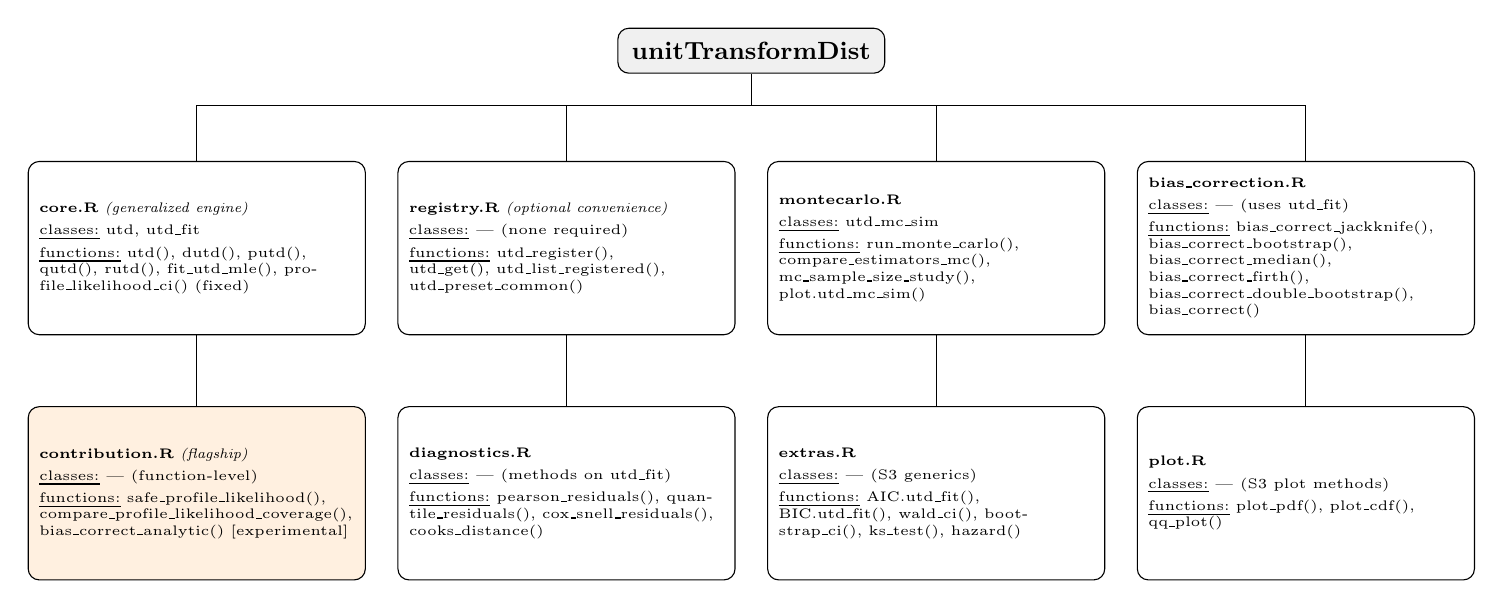
\begin{tikzpicture}[
  every node/.style={font=\tiny},
  cluster/.style={draw, rounded corners, align=left, inner sep=4pt, text width=4.0cm, minimum height=2.2cm},
  root/.style={draw, rounded corners, align=center, inner sep=5pt, fill=gray!12, font=\small\bfseries}
]
% Row 1 (top row): core, registry, montecarlo, bias_correction
\node[cluster] (core)
  {\textbf{core.R} \emph{(generalized engine)}\\[2pt]
   \underline{classes:} utd, utd\_fit\\[2pt]
   \underline{functions:} utd(), dutd(), putd(), qutd(), rutd(), fit\_utd\_mle(), profile\_likelihood\_ci() (fixed)};

\node[cluster, right=0.4cm of core] (registry)
  {\textbf{registry.R} \emph{(optional convenience)}\\[2pt]
   \underline{classes:} --- (none required)\\[2pt]
   \underline{functions:} utd\_register(), utd\_get(), utd\_list\_registered(), utd\_preset\_common()};

\node[cluster, right=0.4cm of registry] (mc)
  {\textbf{montecarlo.R}\\[2pt]
   \underline{classes:} utd\_mc\_sim\\[2pt]
   \underline{functions:} run\_monte\_carlo(), compare\_estimators\_mc(), mc\_sample\_size\_study(), plot.utd\_mc\_sim()};

\node[cluster, right=0.4cm of mc] (bias)
  {\textbf{bias\_correction.R}\\[2pt]
   \underline{classes:} --- (uses utd\_fit)\\[2pt]
   \underline{functions:} bias\_correct\_jackknife(), bias\_correct\_bootstrap(), bias\_correct\_median(), bias\_correct\_firth(), bias\_correct\_double\_bootstrap(), bias\_correct()};

% Row 2 (bottom row), aligned in the same 4 columns
\node[cluster, below=0.9cm of core, fill=orange!12] (contrib)
  {\textbf{contribution.R} \emph{(flagship)}\\[2pt]
   \underline{classes:} --- (function-level)\\[2pt]
   \underline{functions:} safe\_profile\_likelihood(), compare\_profile\_likelihood\_coverage(), bias\_correct\_analytic() [experimental]};

\node[cluster, below=0.9cm of registry] (diag)
  {\textbf{diagnostics.R}\\[2pt]
   \underline{classes:} --- (methods on utd\_fit)\\[2pt]
   \underline{functions:} pearson\_residuals(), quantile\_residuals(), cox\_snell\_residuals(), cooks\_distance()};

\node[cluster, below=0.9cm of mc] (extras)
  {\textbf{extras.R}\\[2pt]
   \underline{classes:} --- (S3 generics)\\[2pt]
   \underline{functions:} AIC.utd\_fit(), BIC.utd\_fit(), wald\_ci(), bootstrap\_ci(), ks\_test(), hazard()};

\node[cluster, below=0.9cm of bias] (plotr)
  {\textbf{plot.R}\\[2pt]
   \underline{classes:} --- (S3 plot methods)\\[2pt]
   \underline{functions:} plot\_pdf(), plot\_cdf(), qq\_plot()};

% Root, centered above row 1
\node[fit=(core)(bias), inner sep=0pt] (row1fit) {};
\node[root, above=1.1cm of row1fit] (root) {unitTransformDist};

% Trunk and bus connecting root to the 4 top-row modules
\coordinate (bus) at ($(root.south) - (0,0.4)$);
\draw (root.south) -- (bus);
\draw (bus -| core.north) -- (core.north);
\draw (bus -| registry.north) -- (registry.north);
\draw (bus -| mc.north) -- (mc.north);
\draw (bus -| bias.north) -- (bias.north);
\draw ($(bus -| core.north)$) -- ($(bus -| bias.north)$);

% Column connectors: each top module to its paired bottom module
\draw[-] (core.south) -- (contrib.north);
\draw[-] (registry.south) -- (diag.north);
\draw[-] (mc.south) -- (extras.north);
\draw[-] (bias.south) -- (plotr.north);

\end{tikzpicture}
\end{figure}
\end{document}
